\section{Gestión de Tareas}
    El usuario tiene a su disposición 2 funciones para la gestión de tareas:
    \subsection{Consultar Tareas}

        Si el usuario da clic a la opción del menú \textit{Ver Tareas}

        \begin{figure}[H]
            \centering
            \hypertarget{VERT}{
\includegraphics[width=0.7\linewidth]{images/Tareas/Vertareaboton}}
            \caption{Opción Ver Tareas}
            \label{VERT}
        \end{figure}

        Se le redirecciona a la siguiente pantalla:
        \begin{figure}[H]
            \centering
            \hypertarget{asignart}{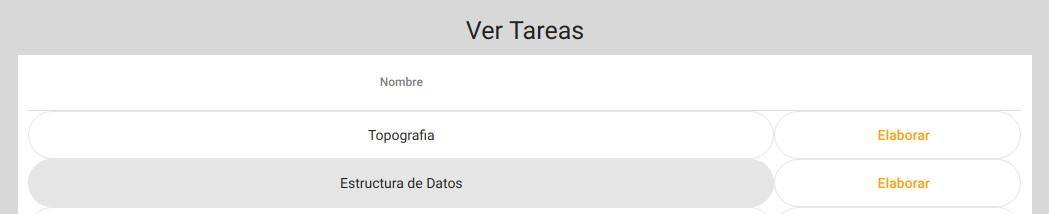
\includegraphics[width=0.7\linewidth]{images/Tareas/Vertareas}}
            \caption{Tabla de tareas}
            \label{asignart}
        \end{figure}
        Donde el usuario ve una tabla con todas las tareas relacionadas con él.



    \subsection{Asignar Tareas}

        Para ello, el usuario da clic en el botón con el icono de una tablita que esta en la fila de la Unidad de Aprendizaje a la que esta asociada la tarea.


        \begin{figure}[H]
            \centering
            \hypertarget{menu}{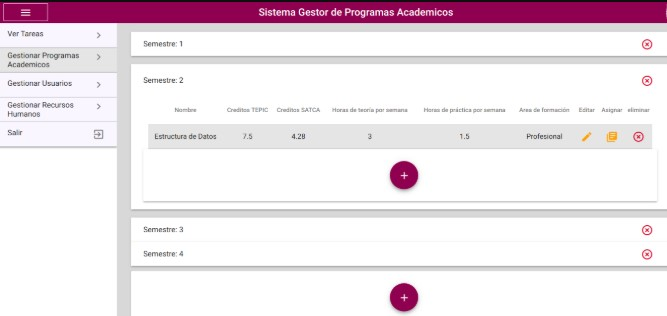
\includegraphics[width=0.7\linewidth]{images/Tareas/Menu}}
            \caption{Menú}
            \label{menu}
        \end{figure}


        \begin{figure}[H]
            \centering
            \hypertarget{boton}{
\includegraphics[width=0.7\linewidth]{images/Tareas/boton}}
            \caption{Botón Asignar}
            \label{boton}
        \end{figure}

        Al hacer esto, el sistema redireccionará al usuario a la pantalla siguiente donde puede seleccionar un usuario para asignarle una tarea.

        \begin{figure}[H]
            \centering
            \hypertarget{asigna}{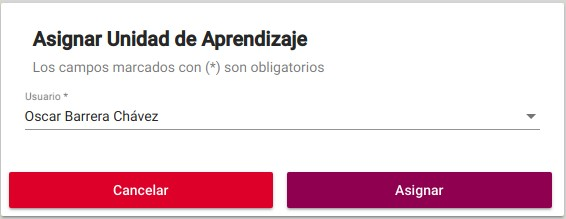
\includegraphics[width=0.7\linewidth]{images/Tareas/Asignando}}
            \caption{Selección de usuario para tarea}
            \label{asigna}
        \end{figure}

       Cuando da click en el botón \IUbutton{Asignar} aparece el siguiente mensaje:
        \begin{figure}[H]
            \centering
            \hypertarget{asignar}{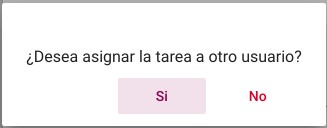
\includegraphics[width=0.7\linewidth]{images/Tareas/Asignarotro}}
            \caption{Selección de otro usuario}
            \label{asignar}
        \end{figure}
        Esto permite asignar una tarea a varios usuarios si selecciona \textit{Si}, en caso de que seleccione \textit{No} regresa a la pantalla de Plan de Estudios.

        Si presiona el botón \IUbutton{Cancelar} le presenta el siguiente mensaje:

        \begin{figure}[H]
            \centering
            \hypertarget{confirma}{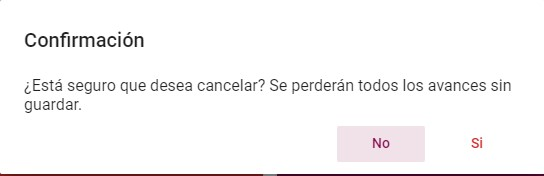
\includegraphics[width=0.7\linewidth]{images/Tareas/Confirmacion}}
            \caption{Mensaje Confirmación}
            \label{conrifma}
        \end{figure}

        Si selecciona la opción \textit{No} puede seguir asignando usuarios a la tarea y si selecciona la opción \textit{Si} pierde todos los avances y regresa a la pantalla de Plan de Estudios.

            \subsubsection{Posibles errores}

                \begin{itemize}
                    \item El usuario no selecciona un usuario para la tarea
                    \begin{figure}[H]
                    \centering
                    \hypertarget{error}{
\includegraphics[width=0.7\linewidth]{images/Tareas/Error}}
                    \caption{Mensaje de Error}
                    \label{error}
                    \end{figure}
                \end{itemize}

